\clearpage
\setcounter{page}{1}
\maketitlesupplementary


\section{Ergänzende Abbildungen}
\label{sec:supp_figures}

\begin{table*}[!t]
\centering
\caption{Übersicht der getesteten Netzarchitekturen. Conv = Anzahl Convolution-Layern, Pool = Anzahl Max-Pooling-Schichten, FC = Anzahl vollständig verbundener Schichten (inkl. Ausgabeschicht), BN = Batch-Normalisierung, DO = Dropout ($p = 0{,}5$).}
\label{tab:architektur_uebersicht}
\resizebox{\textwidth}{!}{%
\begin{tabular}{llccccc}
\toprule
\textbf{Phase} & \textbf{Netzwerk} & \textbf{Conv} & \textbf{Pool} & \textbf{FC} & \textbf{BN} & \textbf{DO} \\
\midrule
1 & Base\_Net                                       & 5 & 2 + GAP & 3 & -- & -- \\
\midrule
2 & Conv\_Net                                       & 8 & 2       & 3 & -- & -- \\
2 & Dense\_Net                                      & 5 & 2       & 7 & -- & -- \\
2 & Pooling\_Net                                    & 5 & 4       & 3 & -- & -- \\
2 & Dropout\_Net                                    & 5 & 2       & 3 & -- & \checkmark \\
2 & BatchNorm\_Net                                  & 5 & 2       & 3 & \checkmark & -- \\
\midrule
3 & BatchNorm\_Dense\_Pool\_Net                     & 5 & 3       & 4 & \checkmark & -- \\
3 & BatchNorm\_Dense\_Pool\_Conv\_Net               & 6 & 3       & 4 & \checkmark & -- \\
3 & BatchNorm\_Dense\_Pool\_Conv\_Dropout\_Net  & 6 & 3       & 4 & \checkmark & \checkmark \\
3 & BatchNorm\_Dense\_Pool\_Conv\_Dropout\_V2\_Net  & 6 & 3       & 4 & \checkmark & \checkmark \\
\bottomrule
\end{tabular}%
}
\end{table*}

% Zusatzmaterial: Tabelle mit Überblick und Validierungs-Accuracy-Verlauf
\begin{table*}[!t]
    \centering
    \caption{Übersicht der Validierungs- und Test-Accuracy der untersuchten
        Netze. Werte als Prozentangaben.}
    \label{tab:results}
    \resizebox{\textwidth}{!}{%
        \begin{tabular}{lcc}
            \hline
            Netz                                           & Val Accuracy (\%) & Test Accuracy (\%) \\
            \hline
            Base\_Net                                      & 57.9              & 59.6               \\
            Dense\_Net                                     & 42.5              & 43.0               \\
            Conv\_Net                                      & 50.7              & 51.2               \\
            Pooling\_Net                                   & 58.0              & 57.4               \\
            Dropout\_Net                                   & 52.5              & 50.4               \\
            BatchNorm\_Net                                 & 82.6              & 79.6               \\
            BatchNorm\_Dense\_Pool\_Net                    & 75.4              & 73.0               \\
            BatchNorm\_Dense\_Pool\_Conv\_Net              & 85.8              & 84.2               \\
            BatchNorm\_Dense\_Pool\_Conv\_Dropout\_Net     & 81.6              & 77.5               \\
            BatchNorm\_Dense\_Pool\_Conv\_Dropout\_V2\_Net & 80.0              & 77.2               \\
            \hline
        \end{tabular}%
    }
\end{table*}

\begin{figure}[ht]
    \centering
    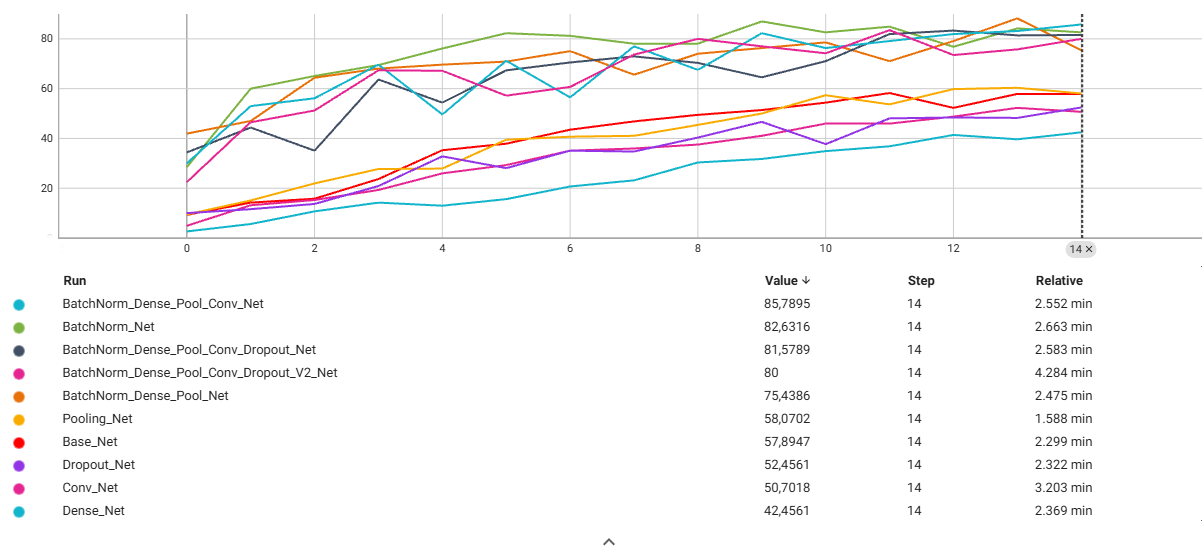
\includegraphics[width=0.9\linewidth]{figures/ValAccuracyAllNets.png}
    \caption{Validierungs-Accuracy über die Trainings-Epochen für alle
        untersuchten Netze. Modelle mit BatchNorm liegen klar über den Netzen
        ohne BatchNorm.}
    \label{fig:val_accuracy_all_nets}
\end{figure}

\begin{figure}[ht]
    \centering
    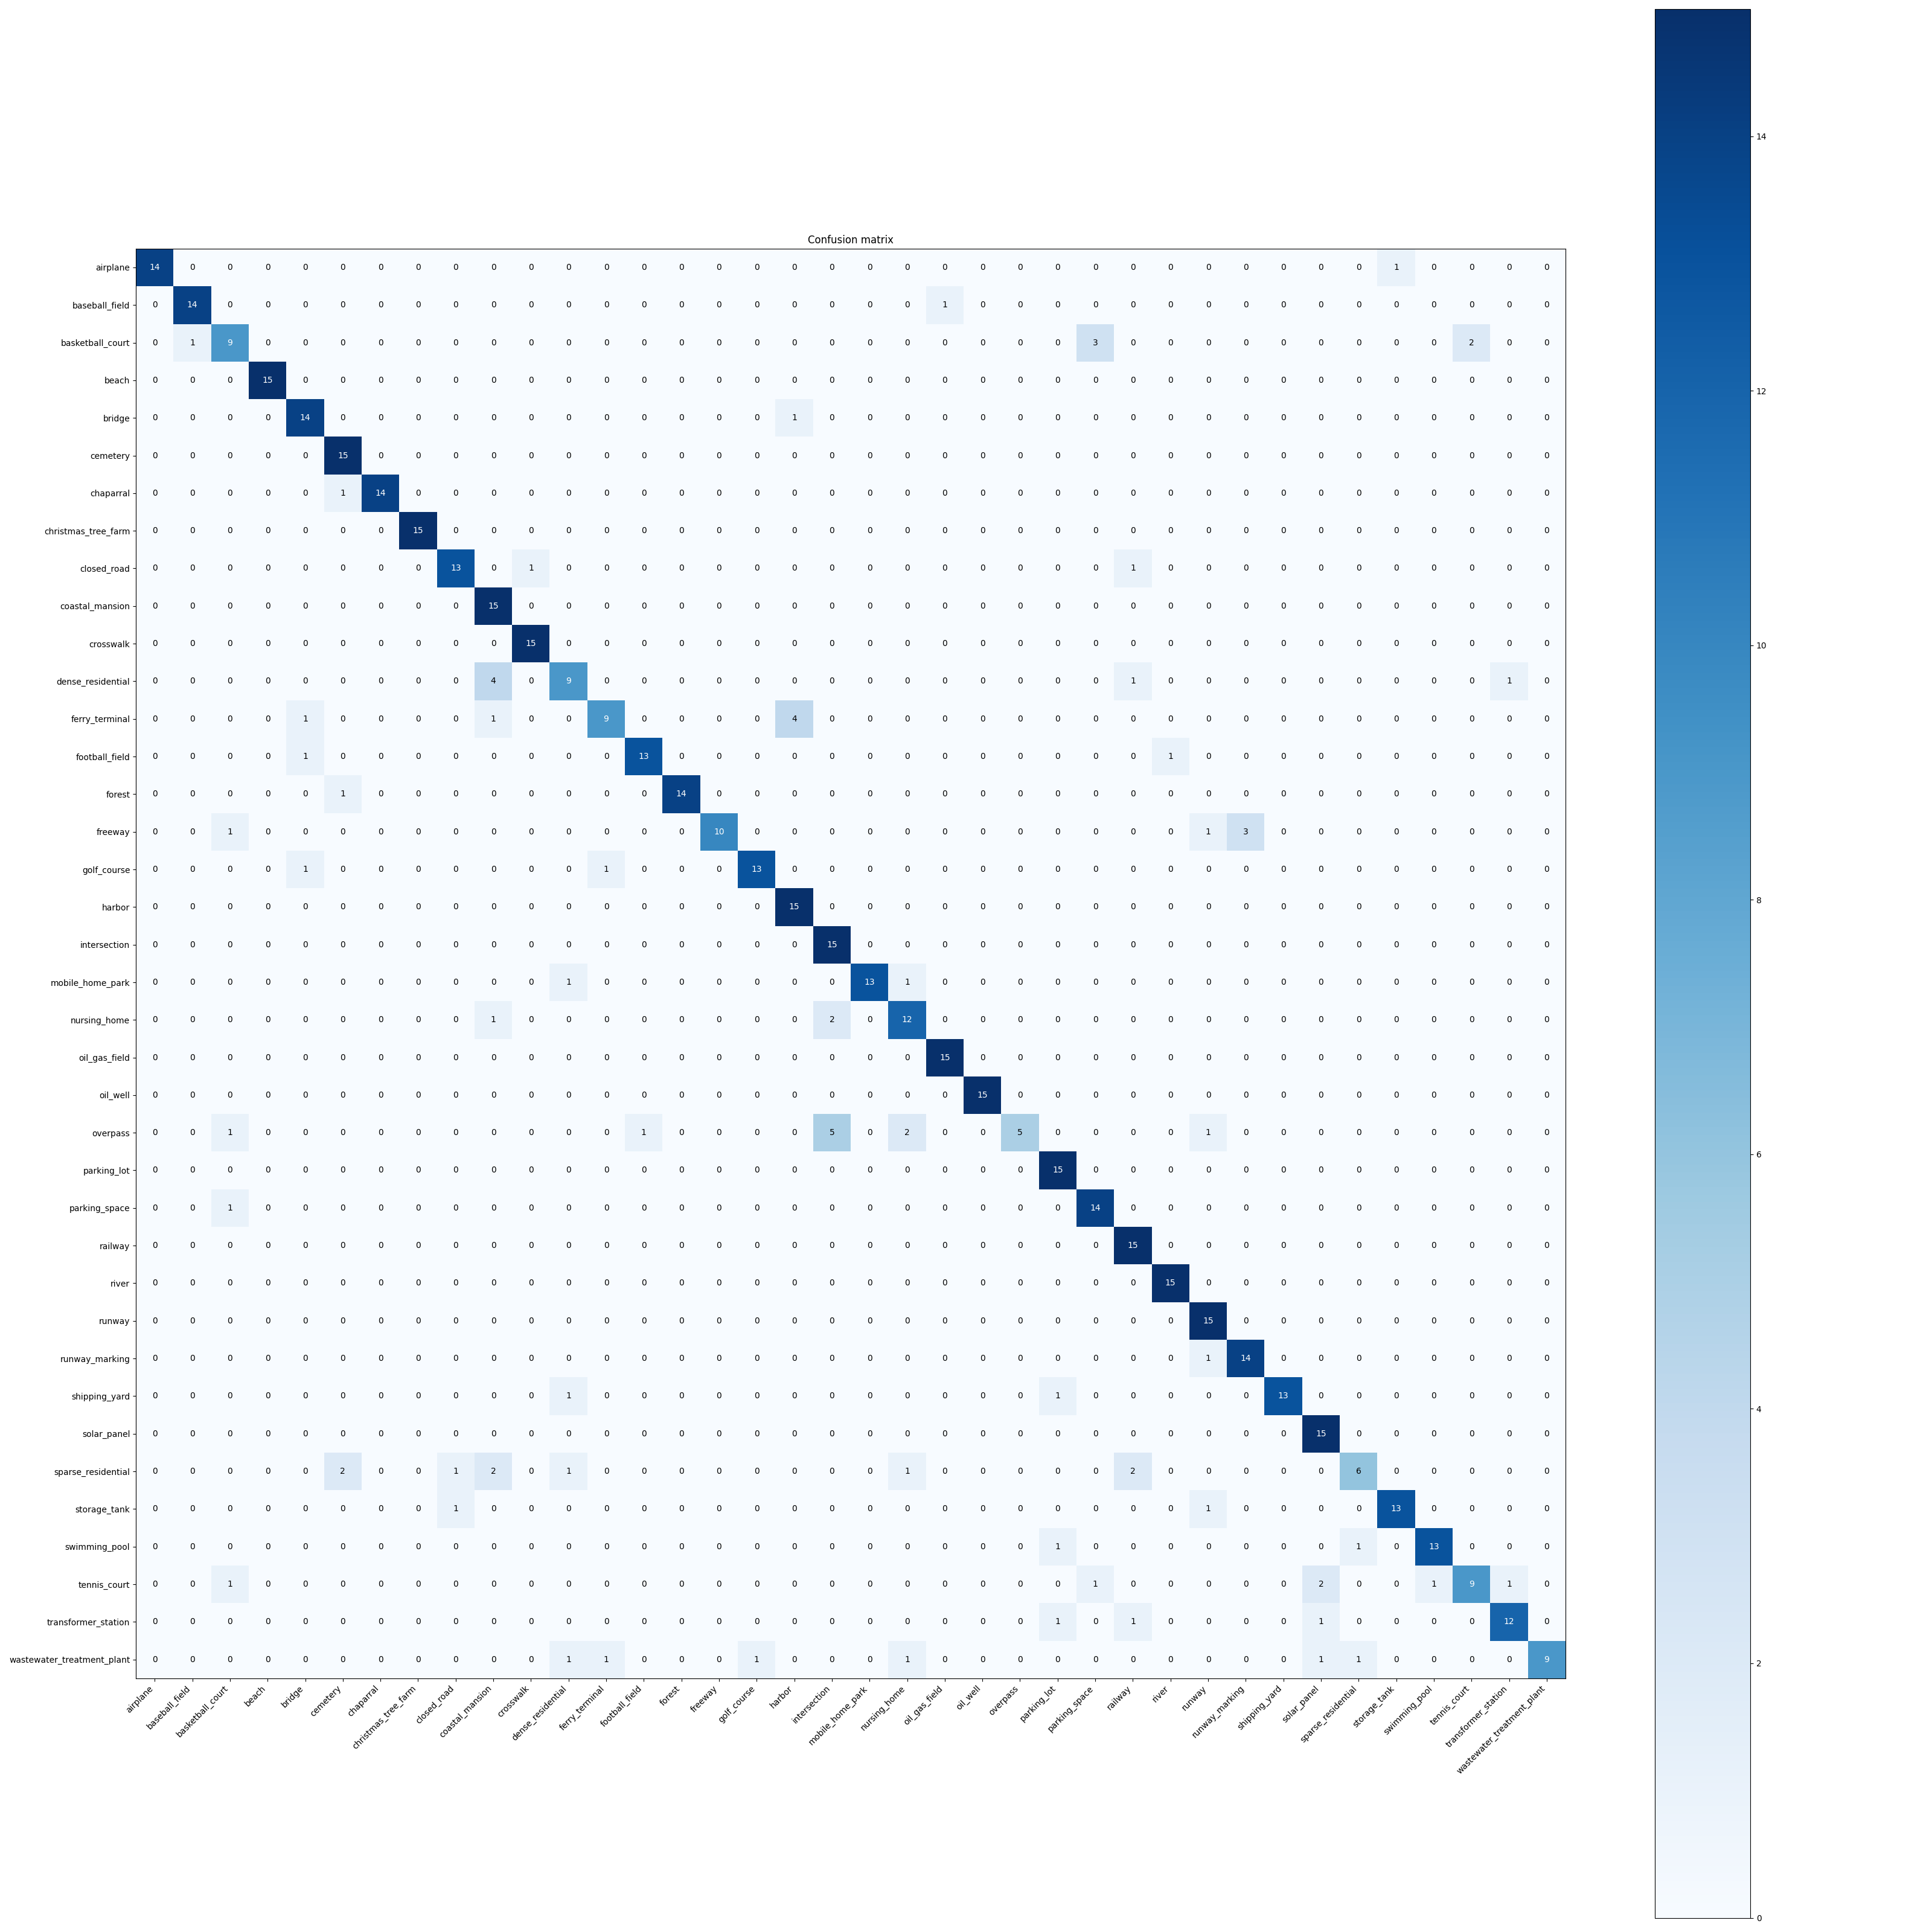
\includegraphics[width=0.9\linewidth]{figures/BestConfusion.png}
    \caption{Konfusionsmatrix des besten Modells. Die Matrix ist fast vollständig
        diagonal; verbleibende Unsicherheiten konzentrieren sich auf visuell
        ähnliche Klassen wie \emph{ferry\_terminal}/\emph{harbor},
        \emph{overpass}/\emph{intersection} und
        \emph{sparse\_residential}/\emph{dense\_residential}.}
    \label{fig:best_confusion}
\end{figure}

\begin{figure}[ht]
    \centering
    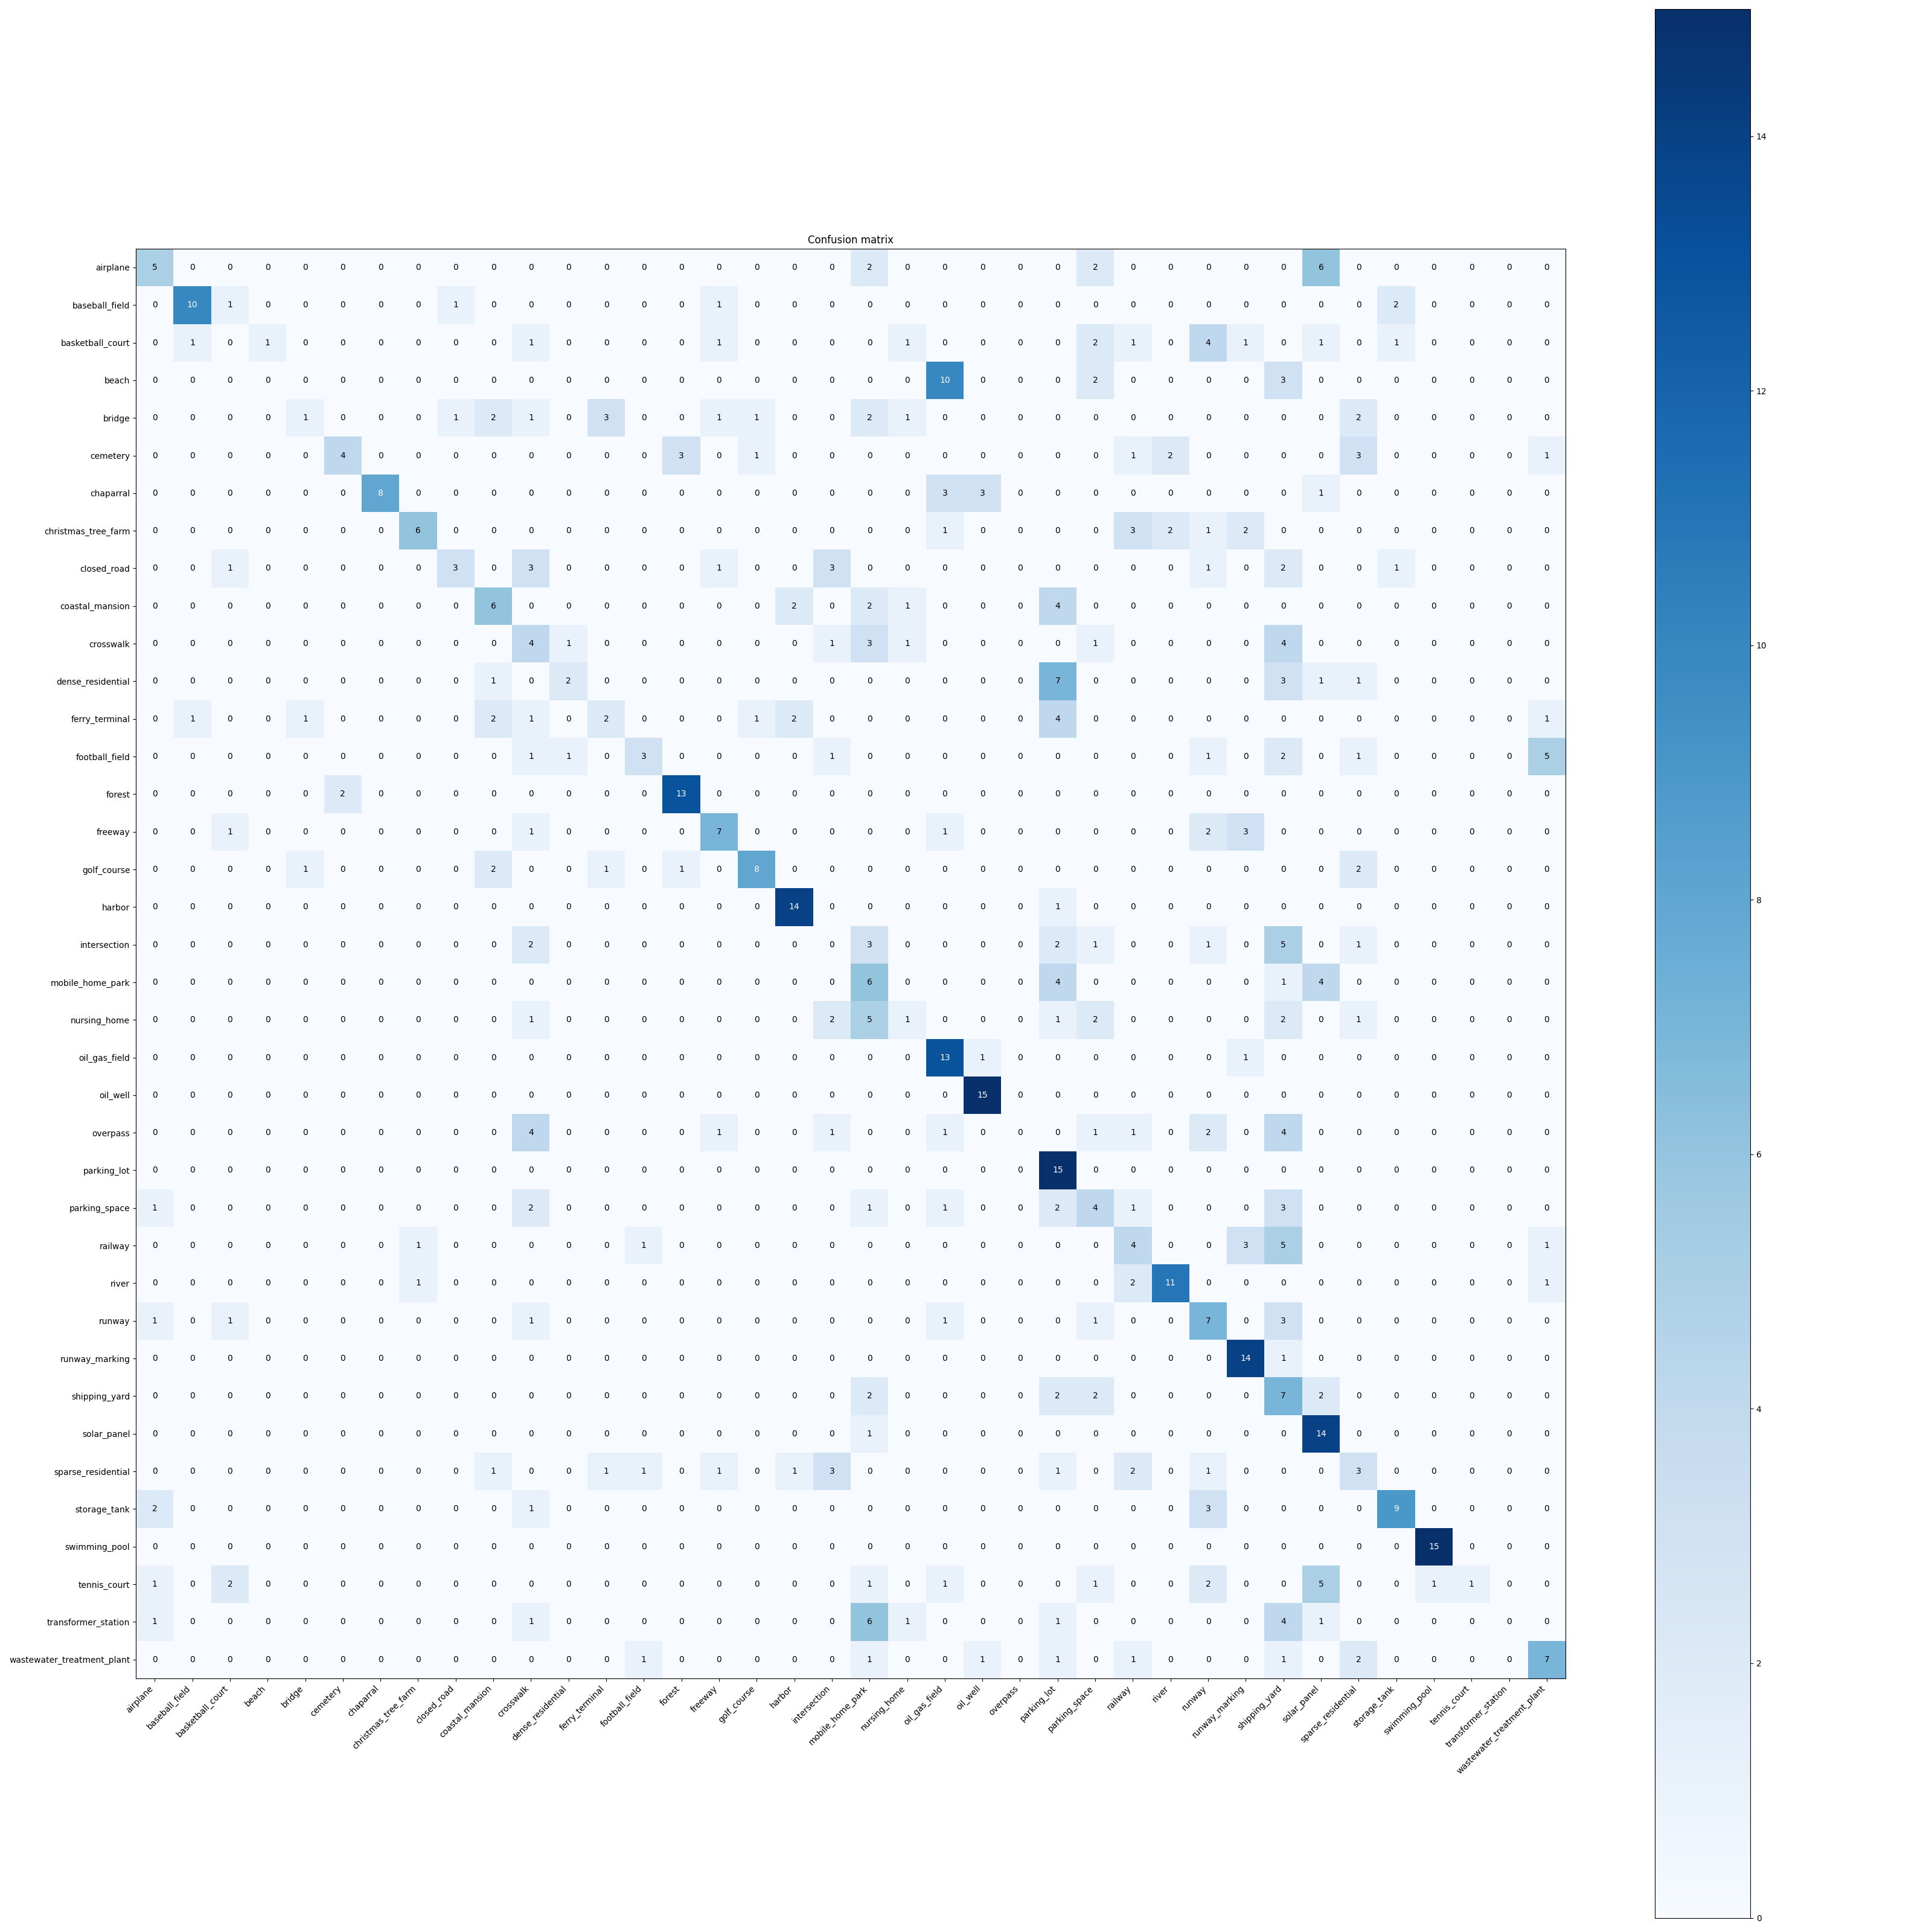
\includegraphics[width=0.9\linewidth]{figures/WorstConfusion.png}
    \caption{Konfusionsmatrix des schwächsten Modells. Im Vergleich zum besten
        Modell ist die Diagonale deutlich unsicherer und die Fehlklassifikationen
        verteilen sich breiter über die Matrix.}
    \label{fig:worst_confusion}
\end{figure}


